\section{Linux Embarcado}

\begin{frame}
    \frametitle{Linux Embarcado}
    \begin{itemize}
        \item Existem aplicações onde somente o uso do 
        microprocessador não é suficiente.
        \item Certas aplicações necessitam de um sistema
        operacional.
        \item O uso de um sistema operacional igual ao dos
        computadores domésticos é inviável pelo excesso de 
        pacotes e funcionalidades desnecessárias.
    \end{itemize}
    

\end{frame}

\begin{frame}
    \frametitle{Linux Embarcado}
    \begin{itemize}
        \item É Necessário criar um sistema operacional customizado
        para o hardware utilizado.
        \item O Linux é comumente utilizado nessas atividades. 
    \end{itemize}
\end{frame}

\begin{frame}
    \frametitle{Linux Embarcado}
    \begin{block}{Linux Embarcado}
        Um sistema Linux Embarcado não se difere conceitualmente 
        de um sistema Linux usado em computadores desktop. A principal
        diferença está na customização e adaptações necessárias para 
        que o Linux seja adaptado ao hardware específico e satisfaça
        os requisitos desejado.
            
    \end{block}    
\end{frame}

\begin{frame}
    \frametitle{Linux Embarcado}
    \begin{figure}[htbp]
        \centering
        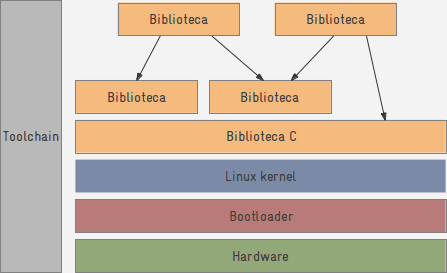
\includegraphics[width=0.9\textwidth]{images/linux-embarcado.png}        
    \end{figure}
    

\end{frame}

\begin{frame}
    \frametitle{Linux Embarcado}
    \begin{enumerate}
        \item    Hardware: o seu produto;
        \item Bootloader: iniciado pelo hardware, responsável pela inicialização 
        básica, carregamento e execução do kernel Linux;
        \item Kernel Linux: núcleo do sistema operacional. Gerencia CPU, memória
        e I/O, exportando serviços para as aplicações do usuário;
        \item Rootfs: sistema de arquivos principal. Possui as bibliotecas do 
        sistema para uso dos serviços exportados pelo kernel, além das 
        bibliotecas e aplicações do usuário;
        \item Toolchain: conjunto de ferramentas para gerar os artefatos de software
        do sistema.
    
    \end{enumerate}
\end{frame}

\begin{frame}
    \frametitle{Linux Embarcado}
    Basicamente, para um sistema Linux Embarcado desempenhar suas funções
    temos que agregar seus diversos artefatos de software - Bootloader,
    Linux Kernel, Bibliotecas, Serviços e Aplicações - para serem executados
    no Hardware alvo. 
    

\end{frame}

